% Options for packages loaded elsewhere
\PassOptionsToPackage{unicode}{hyperref}
\PassOptionsToPackage{hyphens}{url}
%
\documentclass[
]{article}
\usepackage{amsmath,amssymb}
\usepackage{lmodern}
\usepackage{iftex}
\ifPDFTeX
\usepackage[T1]{fontenc}
\usepackage[utf8]{inputenc}
\usepackage{textcomp} % provide euro and other symbols
\else % if luatex or xetex
\usepackage{unicode-math}
\defaultfontfeatures{Scale=MatchLowercase}
\defaultfontfeatures[\rmfamily]{Ligatures=TeX,Scale=1}
\fi
% Use upquote if available, for straight quotes in verbatim environments
\IfFileExists{upquote.sty}{\usepackage{upquote}}{}
\IfFileExists{microtype.sty}{% use microtype if available
	\usepackage[]{microtype}
	\UseMicrotypeSet[protrusion]{basicmath} % disable protrusion for tt fonts
}{}
\makeatletter
\@ifundefined{KOMAClassName}{% if non-KOMA class
	\IfFileExists{parskip.sty}{%
		\usepackage{parskip}
	}{% else
		\setlength{\parindent}{0pt}
		\setlength{\parskip}{6pt plus 2pt minus 1pt}}
}{% if KOMA class
	\KOMAoptions{parskip=half}}
\makeatother
\usepackage{xcolor, color, soul}
\sethlcolor{yellow}
\usepackage[margin=1in]{geometry}
\usepackage{graphicx}
\makeatletter
\def\maxwidth{\ifdim\Gin@nat@width>\linewidth\linewidth\else\Gin@nat@width\fi}
\def\maxheight{\ifdim\Gin@nat@height>\textheight\textheight\else\Gin@nat@height\fi}
\makeatother
% Scale images if necessary, so that they will not overflow the page
% margins by default, and it is still possible to overwrite the defaults
% using explicit options in \includegraphics[width, height, ...]{}
\setkeys{Gin}{width=\maxwidth,height=\maxheight,keepaspectratio}
% Set default figure placement to htbp
\makeatletter
\def\fps@figure{htbp}
\makeatother
\setlength{\emergencystretch}{3em} % prevent overfull lines
\providecommand{\tightlist}{%
	\setlength{\itemsep}{0pt}\setlength{\parskip}{0pt}}
\setcounter{secnumdepth}{5}
\usepackage{amsmath}
\usepackage{amssymb}
\usepackage{float}
\usepackage{titling}
\usepackage[
backend=biber,
natbib=true,
language = english,
doi = false, url = false, isbn = false, eprint = false,
style = apa]
{biblatex}
\usepackage{xcolor}
\ifLuaTeX
\usepackage{selnolig}  % disable illegal ligatures
\fi
\IfFileExists{bookmark.sty}{\usepackage{bookmark}}{\usepackage{hyperref}}
\IfFileExists{xurl.sty}{\usepackage{xurl}}{} % add URL line breaks if available
\urlstyle{same} % disable monospaced font for URLs
\hypersetup{
	pdfauthor={Group II},
	hidelinks,
	pdfcreator={LaTeX via pandoc}}

\DeclareLanguageMapping{english}{english-apa}
\addbibresource{references.bib}

\title{The Price of Air Pollution}
\author{Avdovic Lejla, Blasch Fabian, Schachinger Maximilian, Prinz Martin}

\date{\today}

\begin{document}
	\maketitle
	
	\begin{center}
		
\includegraphics[width = 380pt]{pollution.png} 
	\end{center}
	\thispagestyle{empty}
	\vspace*{30pt}
%	\begin{center}
		\textbf{Abstract} \newline
	Air pollution and its consequences for nature and humanity is an omnipresent global issue, where particularly China stands out. \cite{rasch_under_nodate} reports that coal combustion, industrial production
	and automobile emissions are the main causes for
	air pollution in China. Coal and oil combustion alone account for around 60 percent of $PM_{2.5}$ (Particulate Matter of  2.5 $\mu g$ diameter) pollution in China.
	This paper analyzes the spatial effects of air pollution on the Chinese health care expenditures. We aim to answer the following research question: "To what extent does air pollution and its spatial spillover effects influence health care expenditures in China? A model with a spatial lag in X (SLX) was chosen based on theoretical justifications and a testing procedure, accompanied by a feasible Generalized Least Squares (fGLS) model. 
	The weights matrix chosen to describe the neighborhood structure is contiguity based, since Inner Mongolia, for example, has eight neighbors, whereas Xinjiang has just three. 
	In addition, a robust variance-covariance matrix was included due to heteroscedasticity and serial correlation. The results of the SLX model show that Nitrogen Oxide ($NO$) and Particulate Matter ($PM$)
	increase public health care spending by 0.006 and 0.032, as well as the lag of the second mentioned variable by 0.117 (where only the lag of Particulate Matter is highly significant). For sulphur dioxide ($SO_2$), only the lag has a significant positive effect on our dependent variable of 0.093. In the fGLS model in comparison, the significant positive effect of Particulate Matter of 0.063 and the negative effect of Sulphur of -0.007 remain. We assume that an omitted variable bias is the reason for these counterintuitive results.
%	\end{center}
	\newpage
	\pagenumbering{arabic}
	
	\hypertarget{introduction}{%
		\section{Introduction}\label{introduction}}
	China's recent economic ascent, marked by rapidly growing massive urban centers and surging energy needs, has led to dangerously high levels of air pollution. The research of \cite{chan2008air} identifies China's metropolitan areas as the primary culprits behind the escalating levels of air pollutants. These urban areas account for a significant proportion of direct and indirect sources of emissions, including for example power plants, biogenic, industrial and vehicular sources or domestic heating. 

	Air pollution has been a consistent and pressing issue in China for many years, and its severity cannot be underestimated. Environmental impacts of pollution are not only a concern with regard to climate change but also pose a significant threat to public health. In fact, \cite{maruyama2022air} indicate that over 1.41 billion individuals in China are exposed to $PM_{2.5}$ (Particulate Matter of  2.5 $\mu g$ diameter) levels above 5 $\mu g/m^3$, with 765 million people, or 53 percent of the population, being subjected to health endangering levels exceeding 35 $\mu g/m^3$.
	\cite{song_air_2017} report that the Global Burden of Diseases (GBD) project could assign around 1.6 million deaths in China to air pollution related causes alone in 2015. In addition, persistent and excessive air pollution can be a huge burden to the economy of China: A sustainable development is endangered because natural and human resources are being exposed to dangerous levels of  emissions. This alarming statistic highlights the urgent need for action to protect the well-being of the Chinese population. With increasing health impairments of the population, costs of the public health system are rising. 
	Due to the outdated structure of the social security system in China, which will be discussed in more detail in section \ref{orga}, it is mainly the rural migrants in the urban areas who are suffering the most, as they have to cover the entire costs of medical treatments in urban institutions and pay "out-of-pocket". 
	From a geographical perspective, China features a variety of regions, from rural, mountainous locations to coastal, heavily industrialized clusters. The impact of air pollution may differ between regions and their adjacent provinces.\\ 

	Inspired by the paper "Does industrial air pollution drive health care expenditures? Spatial evidence from China" by \cite{zeng2019does}, our objective is to conduct an independent analysis, which tries to verify their results, identify possible shortcomings and add value to this research field. In their study Zeng and He (2019) employ a spatial lag model with fixed effects in order to disentangle the direct and indirect spatial effects of industrial air pollution on health care expenditures over the period of 2002 to 2014. Their findings reveal that industrial air pollution is a significant contributor to increased health care expenditures not only in the provinces where air pollution is emitted, but also in neighboring provinces. Furthermore, the authors assert that provincial health care expenditures are shaped by a combination of industrial air pollution, health reforms and other socioeconomic factors. These results highlight the importance of considering spatial effects and a range of contextual factors when analyzing the relationship between industrial air pollution and health care expenditures.\\ 
	In this paper we want to adopt the idea of the above mentioned paper and conduct our own spatial analysis using appropriate methods. Our goal is to answer the following research question:

	"\textit{To what extent does air pollution and its spatial spillover effects influence health care expenditures in China?}"

	
	\begin{center}
		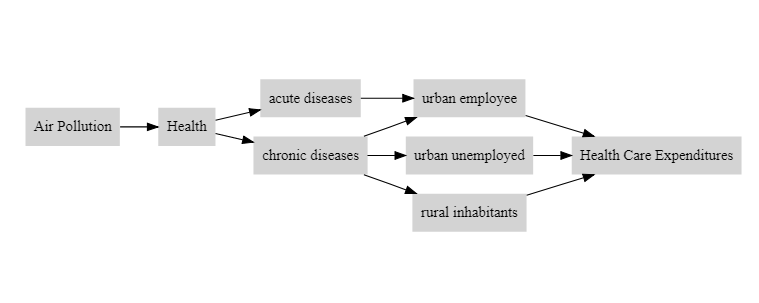
\includegraphics[width=0.9\textwidth]{DAG_true.png} 
		\label{fig:dag}
	\end{center}
	
	Figure \ref{fig:dag} illustrates the channel between Air pollution and Health Care Expenditures as a directed acyclic graph (DAG). Air pollution - namely nitrogen oxide ($NO$), sulfur dioxide ($SO_2$) and Particulate Matter ($PM$) have a direct negative impact on health, as the harmful pollutants penetrate the blood circulation through the lungs and damage other organs. Depending on the duration or concentration of exposure to pollutants, acute diseases such as asthma, bronchitis, respiratory infections, and others can occur. Those can result in long-term consequences, i.e., chronic diseases such as cardiovascular disorders, lung cancer, etc.  
	Depending on which social insurance system a patient is covered - more on this in the section \ref{orga} - outpatient stays are partially covered. In general chronic diseases are partly covered by public expenditures. And so environmental pollution affects the public budget of health care. \\
	This paper is organized as follows. In section \ref{Literature review}, health impacts of air pollution on human health are discussed. This is followed by a brief overview of air pollution policies implemented in the observed period and the organization of the Chinese health care system. The chapter is intended to shed light on the chain of effects of air pollution on government expenditures. More specifically, exposure to air pollution of individuals has negative health effects on them. As a result of deteriorating public health, provincial health expenditures increase. 
	Section \ref{Data} provides a brief description of the data used and an exploratory analysis. 
	Subsequently, in Section \ref{Methodology} the process finding a suitable model and weights matrix as well as the corresponding testing procedure is described, while Section \ref{Results} presents these results. 
	Concluding remarks as well as problems and limitations will be discussed  in Section \ref{Conclusion}. 

	\hypertarget{literature review}{%
		\section{Literature review}\label{Literature review}}
	
	\subsection{Effects of air pollution on health}
	
	Analysing the effect of air pollution on health expenditures implicitly implies the aforementioned causal transition dependencies. Various studies (e.g. \cite{franklin2015air,NYBERG2000,LEL2015}) have identified direct effects of exposure to air pollution on health. 
	
	\cite{franklin2015air} and \cite{fiordelisi2017mechanisms} demonstrate that the risk of cardiovascular diseases and the triggering of acute cardiac events is increased by $PM$ air pollution. The pathways through which this occurs include the generation of proinflammatory or oxidative stress mediators in the lungs that enter the systemic circulation, the direct infiltration of certain particles or components into the cardiovascular tissue, or an imbalance of the autonomous nervous system. In that context, \cite{hoek2013long} quantify the effect of $PM_{2.5}$ long-term exposure by conducting a meta-analytic review of previous studies. Their pooled estimates indicate an increase in all-cause mortality and cardiovascular mortality of six percent and eleven percent, respectively, if increments of $PM_{2.5}$ are increased by 10 $\mu$g/m3. Equivalently, an increase in $NO$ (Nitrogen Oxide) concentration of the same magnitude leads to an increased all-cause mortality of five percent.  
	
	Not only cardiovascular diseases can be enhanced or even caused by air pollution. \cite{KIM2018} found direct impacts of polluted air conditions on lung diseases and pregnancy disorders. According to the authors, even prenatal or perinatal air pollutant exposure can be associated with reduced lung functions of children and can have long-term effects on respiratory health of adults. Additionally, a Swedish study conducted by \cite{NYBERG2000} focused on the relationship between urban air pollution and lung cancer risk. The authors used data from national health registers and modeled air pollution exposure. The results show a significant correlation between higher $NO$ pollution and increased incidence of lung cancer. To be specific, they attributed a higher relative lung cancer risk between 0.8 and 1.6 percent to traffic related $NO$ exposure. 
	
	A study from 2010 conducted by \cite{LEL2015} estimated that between 1.6 and 4.8 million worldwide premature deaths occurred due to outdoor air pollution in 2010 alone, predominately as a result of $PM_{2.5}$ pollution. The largest share of these deaths could be attributed to Asia. 
	
	Additionally, \cite{zhao2019emerging} suggest that based on recent findings air pollution may be involved in the development of autoimmune diseases such as diabetes mellitus, multiple sclerosis, or arthritis. The authors argue that air pollution can cause imbalances in T cells, the production of proinflammatory cytokines, oxidative stress and local pulmonary inflammation. These effects are involved in initiating or aggravating autoimmune diseases. \\ 
	
	To illustrate the magnitude of air pollution-related illnesses, the causes of death by illness patterns provide information. According to \cite{who_nodate} the major premature death causes 2019 in China were cardiovascular diseases totaling 43 percent, followed by malignant neoplasms (26 percent), respiratory diseases (10 percent), unintentional injuries (6 percent) and neurological conditions (4 percent). Other conditions that accounted for between 3 and 1 percent of premature deaths, in descending order, were digestive diseases, genitourinary diseases, respiratory infections, diabetes mellitus and infectious and parasitic diseases. This statistic should illustrate that diseases related to air pollution, such as cardiovascular, cancer or respiratory diseases, make up for an substantial share of public health issues. \\ 

	
	\subsection{Air pollutions policies from 2011 to 2018}
	
	Air pollution in China has been a major public health problem for many years. However in recent years the government has taken various measures to address the issue. One of the main focuses of these measures has been to reduce emissions of particulate matter, sulfur dioxide and nitrogen oxides. 
	According to \cite{CHINA2013}, in 2013, prompted by a period of heavy smog in eastern China, the government introduced an "Air Pollution Control Action Plan" to combat air pollution, which included specific targets for reducing particulate matter, sulfur dioxide, and nitrogen oxide emissions. More specifically, targets included, among others, reducing $PM_{10}$ concentrations in cities by more than 10 percent and reducing $PM_{2.5}$ concentrations in the Beijing-Tianjin-Hebei, Pearl River Delta and Yangtze River Delta regions by  around 25, 15 and 20 percent, respectively. 
	
	Furthermore, the 13th Five-Year Plan (2016-2020) published by \cite{CHINA2016} also set a target to further reduce $PM_{2.5}$ concentrations in areas heavily affected by air pollution by 18 percent until 2020. Targets have also been set for further reducing $SO_2$ and $NO$ emissions by both 15 percent compared to 2015 levels. 
	
	\cite{HUANG2018e313} indicate in their analysis, in which they map the national air quality in 74 cities that the issued Air Pollution Prevention and Control Action Plan (APPCAP) in 2013 has shown effect. Between 2013 and 2017 $PM_{2.5}$ concentrations have reduced in average by about 33 percent, and $PM_{10}$ concentrations by about 28 percent. $SO_2$ concentrations have reduced as well with an average reduction of about 54 percent. $NO$ emissions, however, have not significantly decreased. 
	
	In addition, new air quality standards were set in February 2012. These were initially enforced in large cities and their surrounding areas in the following years until they were implemented nationally in 2016. According to the \cite{Transport2012} new standards set stricter limits for air pollutants such as particulate matter, sulfur dioxide, nitrogen oxides and ozone to better protect public health. Chinese authorities have also introduced new monitoring and reporting technology to ensure that air quality is measured and monitored in every part of the country. Companies that violate the new standards can be fined or even shut down. 
	
	In their article \cite{ijerph13121219} summarize that a number of measures have been taken by the Chinese government from 2011 to 2019 to reduce air pollution, including stricter emission standards for vehicles, power plants and industrial facilities, and the closure or upgrading of older, heavily polluting factories, which were partially effective. 
	
	\begin{center}
	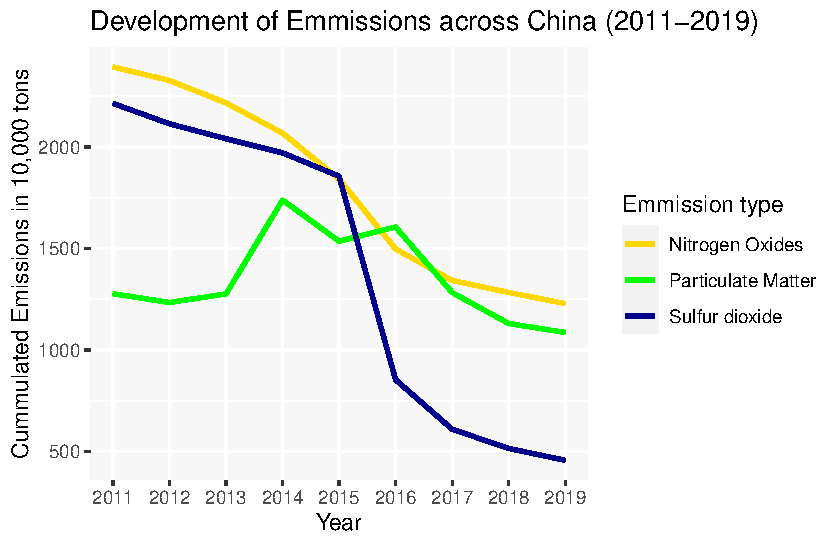
\includegraphics[width=0.6\textwidth]{Development of Emmissions China total.pdf} 
	\label{fig:Cummulated Emmissions}
	\end{center}

	Figure \ref{fig:Cummulated Emmissions} displays China's total emission volumes of $PM$, $SO_2$ and $NO$ pollutants. Similar to the literature, we observe a strong downward trend in emission levels of all three air pollution variables in the data. It seems that the previously discussed measures are showing an effect in China. 

	\subsection{Organization of the Chinese Healthcare System} \label{orga} 
	Since the late 1990s, which are also considered to be the years of the opening and globalization of China according to \cite{kanbur_fifty_2005}, in which the country developed from a centralized to an open market economy, there have been several economic reforms in the country, including in the health care system.
    \cite{shi_health_2018} describe that due to the reforms the health care system became a market-based. Furthermore, the rural medical insurance almost completely collapsed as the dissolution of communes led to insufficient financing. In 2003, around 78\% of the whole population was not covered by medical insurance any kind. In the early 1980s, private medical care insurance was introduced, but it was only available to a limited extent. 
	As China focused on implementing universal coverage - between 2003 and 2008 - several variations of medical insurance were introduced. As a result, the percentage of uninsured in China decreased to 12.9%. 
	 \cite{hougaard_chinese_2011} state that the Chinese Central Government was heavily reduced from healthcare meaning the provinces are now responsible for financing and administering the Health Care System. \\
	Before we delve deeper into the organization of the Chinese health care system, it is worth mentioning how social benefits are allocated in China.
	The \textit{hukou system} is the official residence registration system on household level in China, where individuals are assigned to a permanent residence.
	\cite{noauthor_oecd_nodate} report that workers from rural regions who migrate to urban areas face discrimination in accessing services due to not having an urban residency registration. 
	\cite{liu_institution_2005} describes  that originally the hukou system was established in Chinese cities to "maintain social peace and order, ensure the security of the people, and protect their freedom of residence and movement." 
	However, this changed in 1955 as there was a strong influx of farmers into the cities. The government expanded as a response the hukou to also include rural regions.  
    The registration system was now considered a government instrument to not only control but also mitigate migration flows between urban and rural areas. After that any change of residence required an administrative authorization. It was essential from the point of view of the centrally planned government to distribute human resources across various geographic locations. Therefore, from a contemporary perspective, the hukou system could also be seen as a relic of the centrally planned economy.

	The Chinese health care system is characterized by the division of the population between two groups: The proportion of the population living in the urban and rural areas.
	\cite{shi_health_2018} have provided a broad overview: The so-called Urban Employee Basic Medical Insurance (UEBMI) program for urban workers was implemented following pilot projects in several urban regions in the 1990s.
	Between 2003 and 2008, the New Rural Cooperative Medical Scheme (NRCMS) was also implemented for the rural population, at first only in a few regions, but later expanded to include all rural areas in China.
	However, even after the introduction, some urban residents without employment contracts, such as children, students, people with disabilities, etc., remained uncovered. The  Urban Resident Basic Medical Insurance (URBMI) was introduced across the nation in 2009 to provide coverage for urban citizens who did not qualify for UEBMI.
	The aforementioned three basic insurance plans in China maintained to cover over 95\% of the population.

	
	\section{Data} \label{Data}
	
	For our analysis, we use data retrieved from the \cite{NBSChina}. The data was compiled from an extensive database. It provides data on government spending, air pollution, and various socioeconomic factors on a provincial level. In total we use a balanced panel of yearly data from 2011 to 2019 of 31 provinces. In advance, we excluded autonomous regions such as Hong Kong, Macau or Taiwan, for which data were also partially available. The dependent variable of our analysis "Local Governments Expenditure on Medical and Health Care" includes all conceivable kinds of government spending, including for example health care management and services expenditures, disease prevention and motherhood expenditures as well as rural health spending. The variable is measured in 100 million Yuan. Additionally, we extracted three different pollution variables, namely particluate matter, sulfur dioxide and nitrogen oxides emissions volumes, which are measured in 10000 tons. However, no information was provided on whether the data was smoothed regionally. Furthermore, include various socioeconomic control variables in our analysis. ariables such as the population shares of different age groups (0-14, 15-65, 65-), which were collected through random sampling, the average disposable household income for each urban and rural population in the province, the coverage rate by forest in the region, and the proportions of urban and rural population in the region serve as important control variables in our analysis. 
	In addition, we included other variables in our initial models, but at a certain point we no longer considered them important because the influence of these variables were either already covered by other variables or they offered very little explanatory value for our analysis. These include the the gross regional product, total local government expenditures and various key figures relating to the health system.
	
	\subsection{Exploratory Analysis}
	Now that we have established the source as well as the meta information. We will concisely examine the variables of highest relevance. The nature of our dataset does unfortunately not allow for a static representation that could display information of all provinces across time. Accordingly, we will focus on the values of our dependent variable as well as all emissions variables based on the beginning of our time series in 2011 and the end in 2019. In particular, the focus will be on the values in the different provinces at those points in time as well as their spatial interaction measured via the local Morans's I. Starting with our dependent variable we observe that the health care expenditures across all provinces increased across the eight years in our sample, this is not very surprising as China's population grew quite drastically in this time frame and accordingly the health care expenditures grew as well.
	\begin{center}
		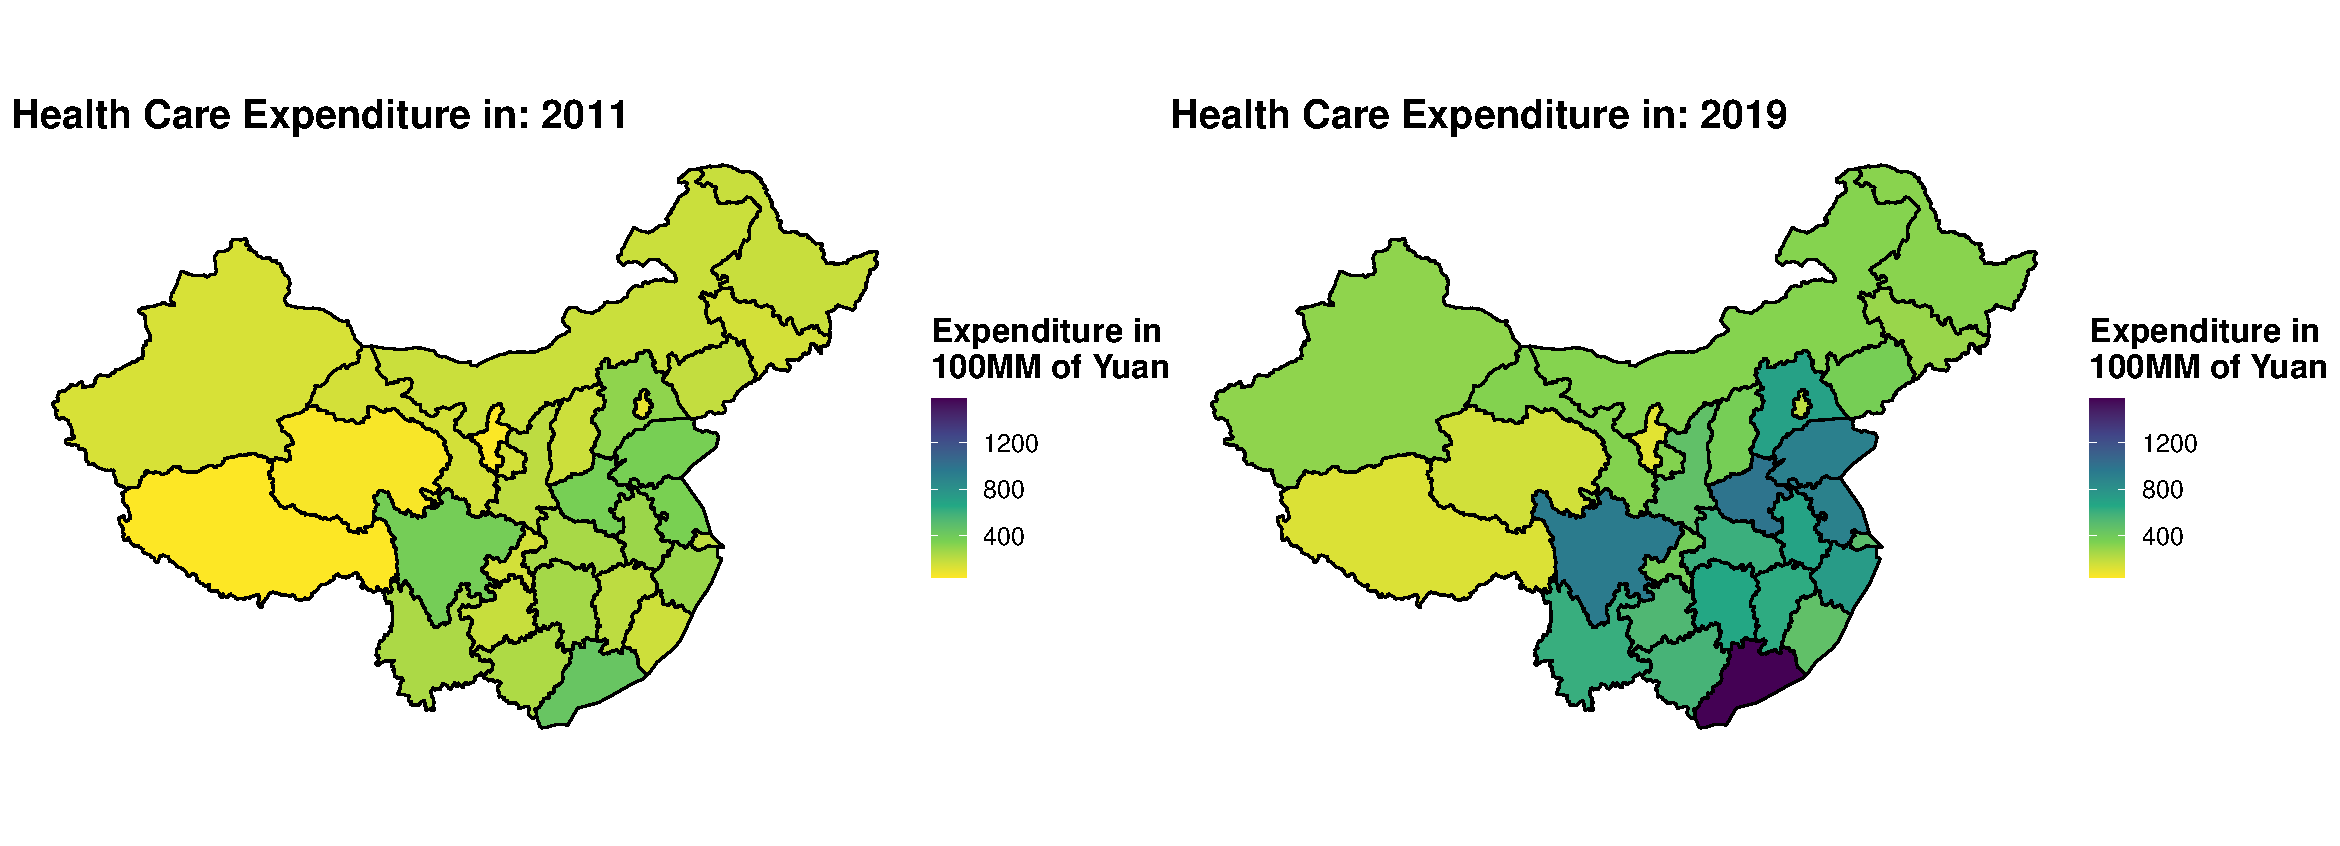
\includegraphics[width = 440pt]{Health_Care_Expenditures_comp.pdf} 
	\end{center}
	\begin{center}
		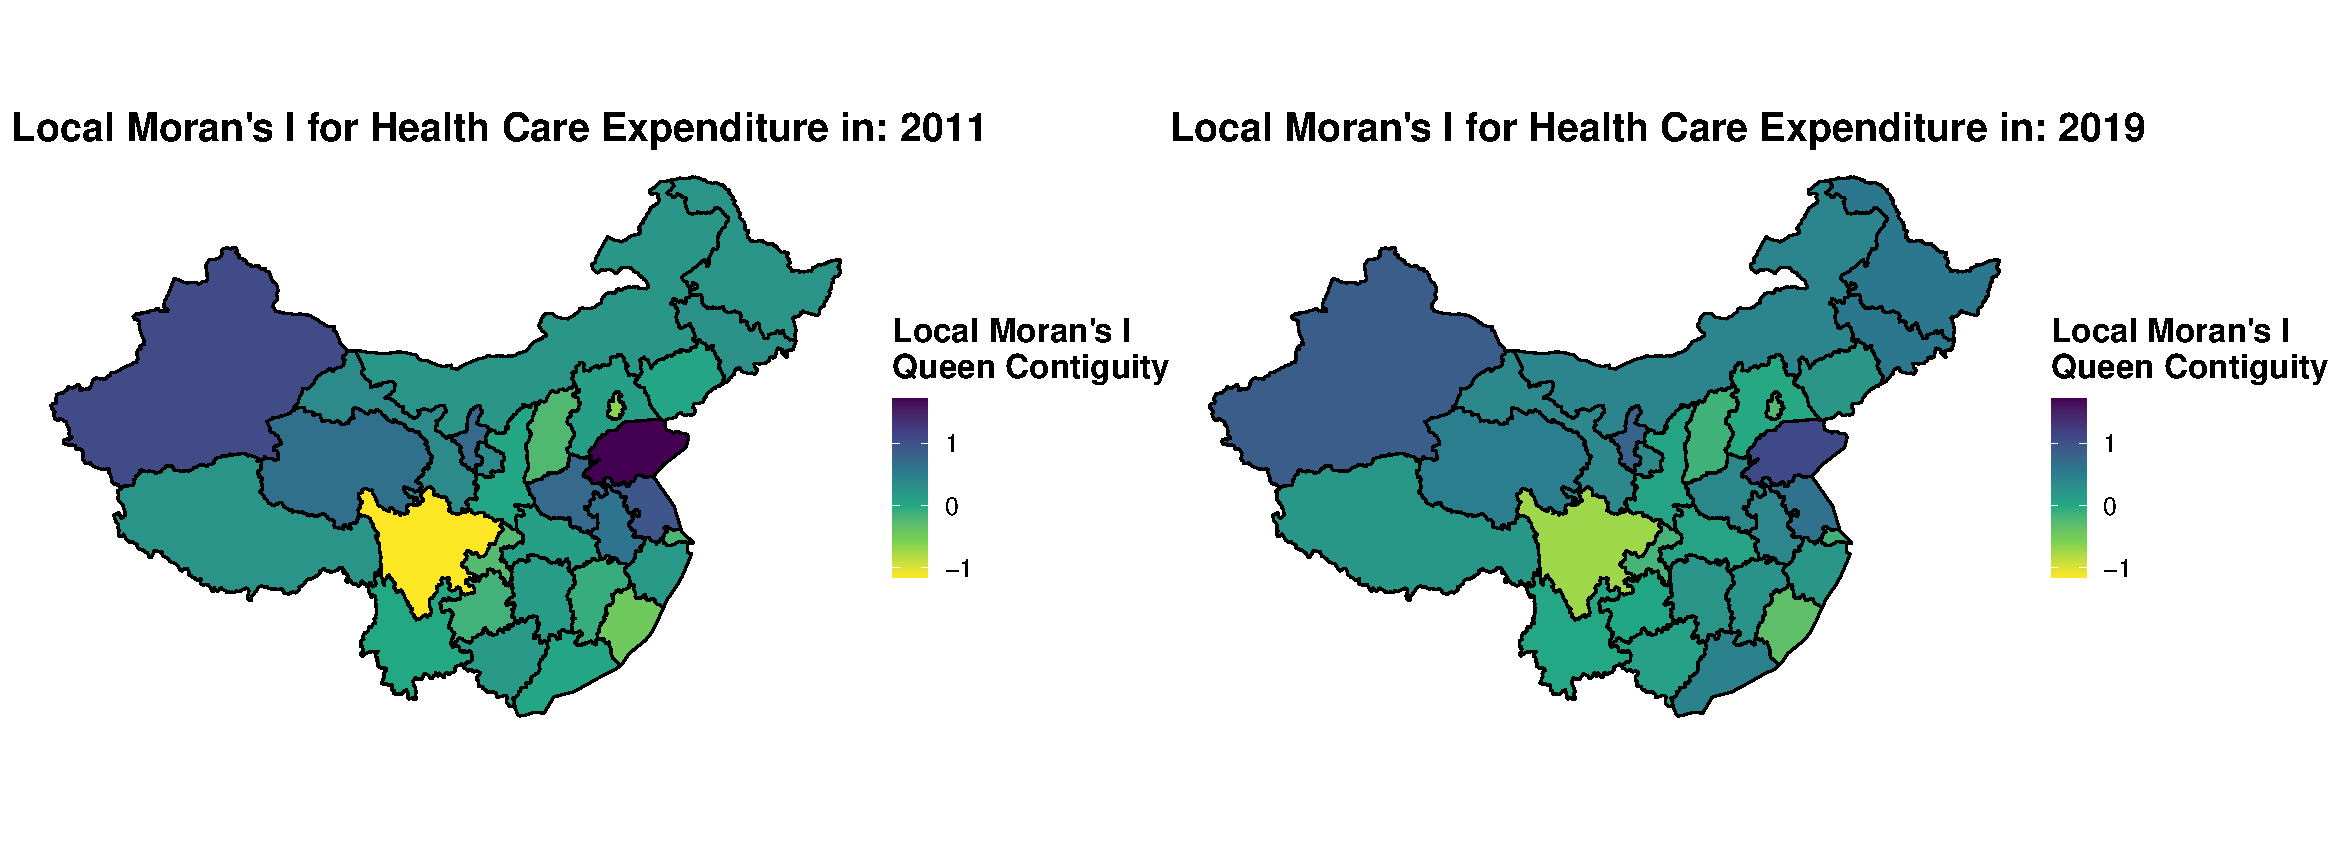
\includegraphics[width = 440pt]{Ii_Health_Care_Expenditures_comp.pdf} 
	\end{center}
	Further, when examining the spatial interaction we see that it changed quite drastically from 2011 to 2019. This is at least to some degree caused by the increased heterogeneity across provinces when it comes to health care expenditure at the end of our time frame.\\
	As a representative for our pollution variables, Particulate Matter emission developments are displayed below. We can immediately tell that Particulate Matter emissions for most provinces and especially for Hebei, the province that surrounds Beijing, decreased quite substantially from 2011 to 2019. However, this does not seem to be the case for two special cases located in the north-east of china. Both in Jilin and in Inner Mongolia, the amount of Particulate matter emission increased.
	\begin{center}
		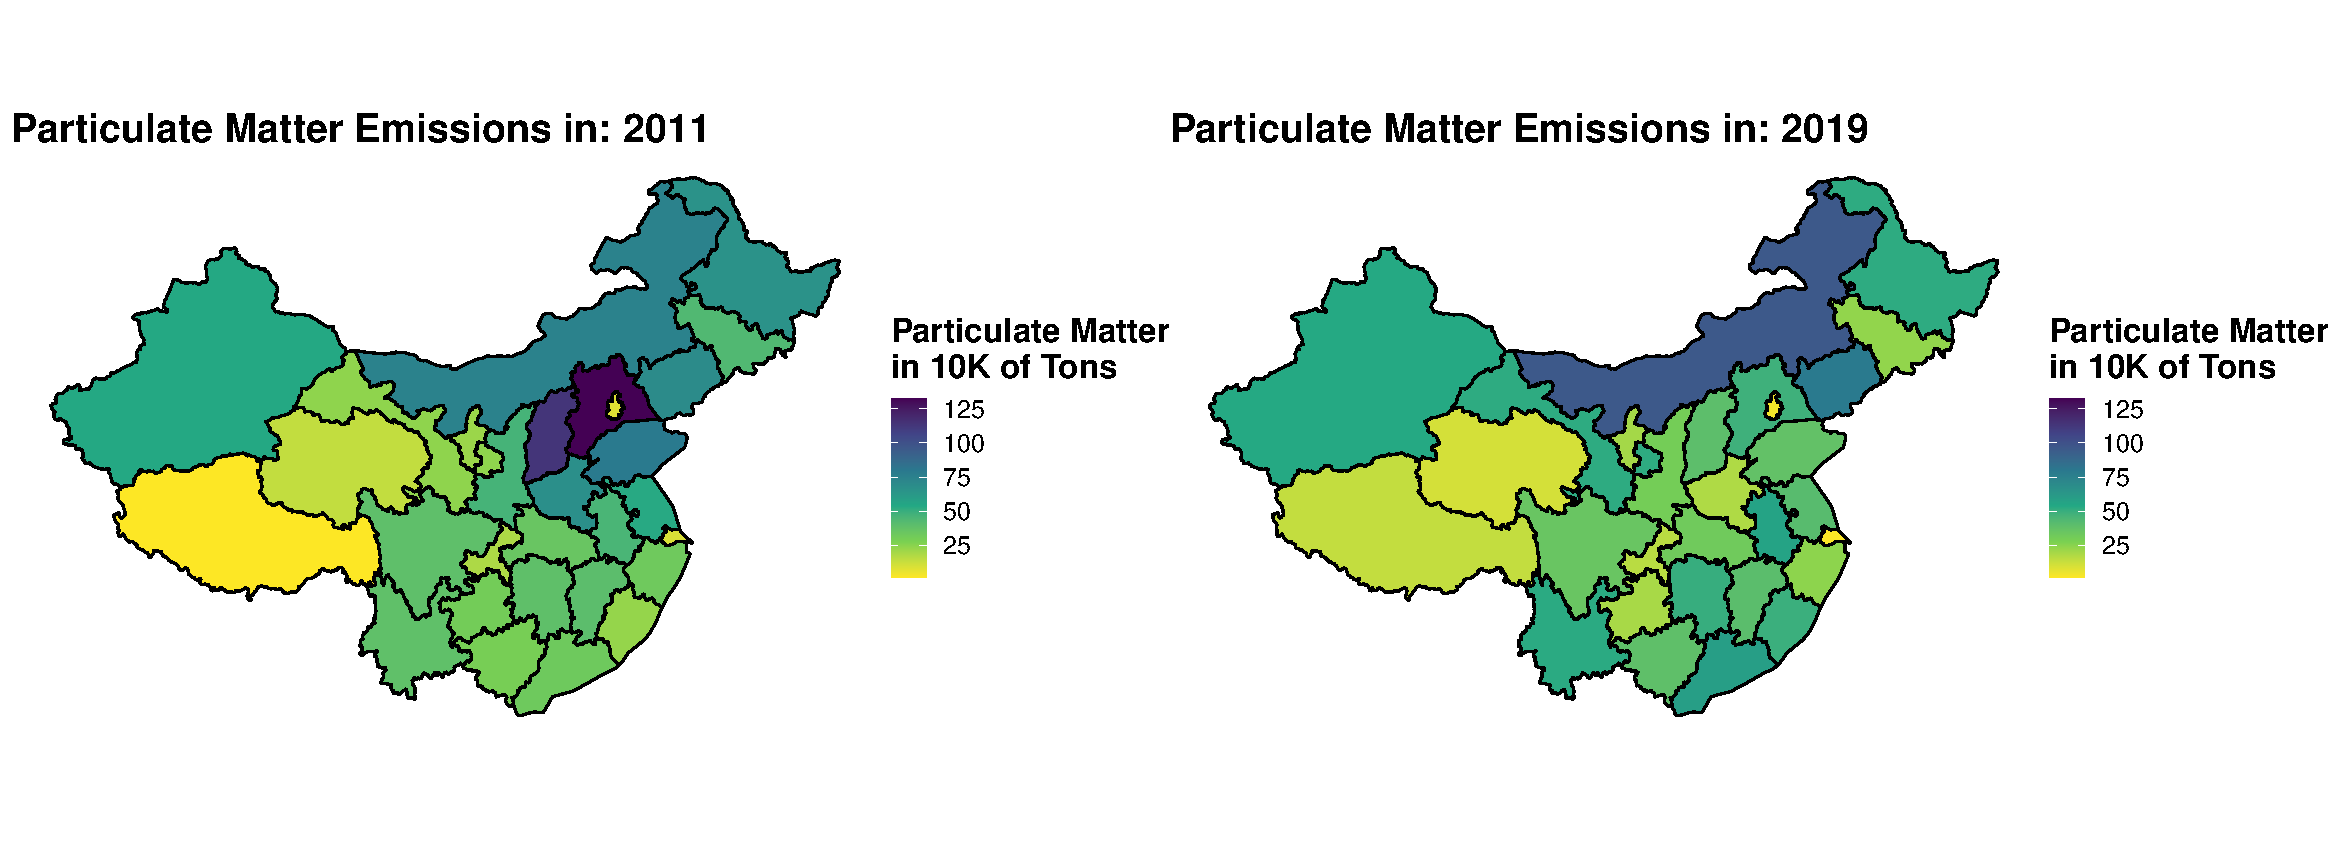
\includegraphics[width = 440pt]{Waste_Gas_Emissions_Particular_Matter_comp.pdf} 
	\end{center}
	\begin{center}
		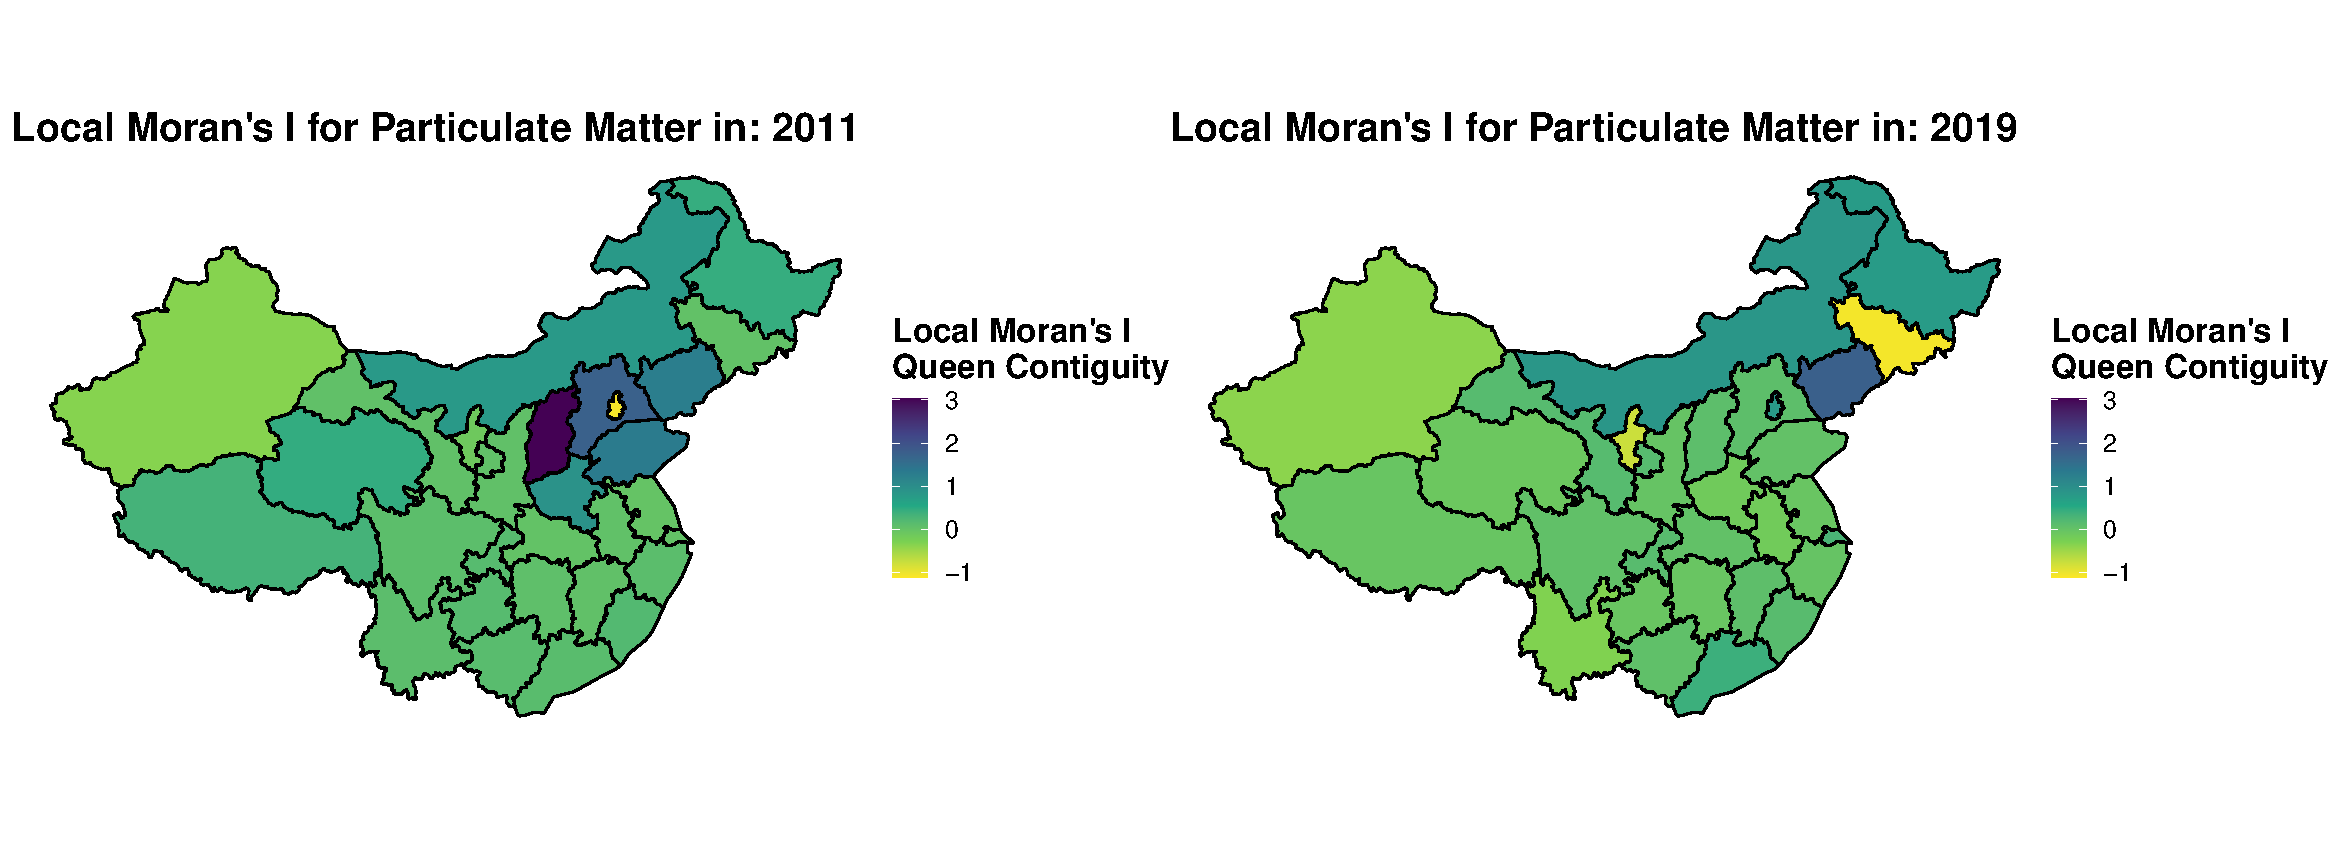
\includegraphics[width = 440pt]{Ii_Waste_Gas_Emissions_Particular_Matter_comp.pdf} 
	\end{center}
	In regard to the spatial interaction, we can observe that the Moran's I also changed quite significantly, again a large part of those changes may be attributed to strong decreases in emissions in provinces around Beijing. The maps for the remaining variables have been added to the appendix.

	\section{Methodology} \label{Methodology}
	A vital part of a spatial analysis is the determination of a weights matrix that describes the dependence structure of the observations. For our analysis we elaborated the use of k-nearest neighbors, contiguity and a inverse distance type of W-matrix. We decided upon the use of a first (queen) contiguity approach, where every province, that shares a direct border will be considered a spatial neighbor. The reason for this approach is that it describes a very simple and less error prone dependence structure. The use of k-nearest neighbors would be for example problematic in a province like Inner Mongolia, where 8 other provinces share a border but only k would be selected. The use of a inverse distance based weight would also be problematic as it is not known where emission creating facilities are located. \\
	As already discussed in section \ref{Literature review}, the possibility of a Spatial Autoregressive Process (SAR) is rather unlikely considering the hukou system. We therefore excluded the possibility of a SAR component before using statistical testing to determine the final model.\\
	We started the testing procedure by using the (Spatial) Hausmann Test to decide whether fixed or random effects suit the data better. The test strongly indicated the usage of a fixed effects model over time, which is in line with the intuition as China's provinces are heterogenerous and eliminating time constant features such as geographic differences seems like a reasonable approach.\\
	In the following, a Lagrange Mulitplier Test was utilized to decide whether a Spatial Error Model (SEM) would be necessary. We could not reject the $H_0$ of a OLS model. Therefore, we continued to use a Spatial Lag in X (SLX) model, whose lag components can directly be tested by t-tests. The inclusion of a SLX component comes from the fact that air pollution of one province is likely to influence air pollution of neighboring provinces. But, as already discussed in section \ref{Data}, it is not known whether the emission variables are measured as total emissions created in a province or if some smoothing procedure of the data was already applied. If the latter would be the case, the use of a SLX model would be redundant, as it would mostly report the effect of the smoothing process. Nevertheless, introduction of spatial lags of air pollution will not cause any harm other than potential multicollinearity issues if they are in fact redundant.\\
	As a next step we tested the possible presence of heteroscedasticity and serial correlations in the error terms. For the former a Breusch-Pagan test was used to test, where we could reject the Null-Hypothesis of homoscedastic errors. For the latter a Durbin-Watson test was conducted. The test strongly suggested serial correlation. As a result, we used a robust variance-covariance matrix in order to account for this error structure and improve the reliability of our results\\
	For the identification of the model, a general-to-specific approach was used, where we started with all reasonable variables and potential lags and then eliminated them iteratively with the use of t-tests.\\
	As a robustness test for our results, we used a feasible Generalized Least Square model. Very similar to the SLX model we use a robust variance covavariance matrix that is corrected for heteroscedasticity and serial correlation. Also, the most general model is assumed again and variables are eliminated one-by-one.\\
	Some variables of interest are in monetary terms. To account for growth in these variables due to increased prices we adjust every monetary variables (X) by the general consumer price index (CPI)
	$$\widetilde{X} = \frac{X}{CPI/100}.$$
	The CPI is divided by 100 as it is reported with baseline value 100.\\
	Additionally, on every variable a logarithmic transformation was used. The reason for this is twofold. To begin with it might further help with the heteroscedastic and serially correlated errors and therefore provide more reliant estimates. And it also helps to make the interpretation of the estimates more intuitively. One exception to this procedure is the share of working population, as this variables already presents a share of the whole population, a further transformation would make its interpretation meaningless.\\
	
	
	
	\section{Results} \label{Results}
	
	As previously outlined, the models presented in the table below were obtained using the general to specific model selection procedure. Starting from the model with all controls, statistically insignificant explanatory control variables were subsequently removed one at a time. During this process, the sign as well as the significance of our pollution variables were very sensitive to small changes in the model, i.e., we observed large changes in obtained estimates over a single iteration of the general to specific selection procedure. Accordingly, the presented results are to be interpreted cautiously. The unstable coefficient estimates are most likely caused by a combination of highly collinear explanatory variables and the absence of important variables that drive health care expenditures in our model.\\ Nevertheless, some key takeaways can be made. We observe that in our model, which does not contain spatially lagged variables, that Particulate Matter emissions have a significant effect while in the SLX model this is not the case. This might be due to the mentioned multicollinearity problems, as all pollution variables exhibit a positive spatial correlation. The negative and significant effect of Sulphur Gas emissions, is most likely also a result of the multicollinearity in our model. Especially, given that the spatial lag features a positive and significant coefficient, there is no sensible interpretation to be made. The key takeaway should thus be, even though we find a positive and significant effect of Particulate Matter emission (fGLS) on Health Care Expenditure, the result is both unstable over iterations in our model selection procedure and also across model types. Further, given our modelling and identification strategy, we may not claim that the results represent a causal relationship between the examined variables.
	\begin{table}[H] \centering 
		\caption{Results fGLS \& SLX} 
		\label{} 
		\begin{tabular}{@{\extracolsep{5pt}}lcc} 
			\\[-1.8ex]\hline 
			\hline \\[-1.8ex] 
			& \multicolumn{2}{c}{\textit{Dependent variable:}} \\ 
			\cline{2-3} 
			\\[-1.8ex] & \multicolumn{2}{c}{ } \\ 
			\\[-1.8ex] & fGLS & SLX\\ 
			\hline \\[-1.8ex] 
			log(Disposable Income per Capita Rural) & 1.072$^{***}$ &  \\ 
			& (0.067) &  \\ 
			& & \\ 
			log(Disposable Income per Capita Urban) &  & 1.180$^{***}$ \\ 
			&  & (0.081) \\ 
			& & \\ 
			log(Forest Coverage Rate) & 0.490$^{***}$ & 0.287$^{**}$ \\ 
			& (0.102) & (0.144) \\ 
			& & \\ 
			log(Urban Population) & 0.308$^{**}$ & 0.504$^{***}$ \\ 
			& (0.145) & (0.135) \\ 
			& & \\ 
			log(Waste Gas Emissions Nitrogen) & $-$0.045 & 0.006 \\ 
			& (0.035) & (0.041) \\ 
			& & \\ 
			log(Waste Gas Emissions Particulate Matter) & 0.063$^{***}$ & 0.032 \\ 
			& (0.024) & (0.023) \\ 
			& & \\ 
			log(Waste Gas Emissions Sulphur) & $-$0.007 & $-$0.063$^{**}$ \\ 
			& (0.016) & (0.028) \\ 
			& & \\ 
			log(Waste Gas Emissions Nitrogen Lag) &  & $-$0.111 \\ 
			&  & (0.088) \\ 
			& & \\ 
			log(Waste Gas Emissions Particulate Matter Lag) &  & 0.117$^{***}$ \\ 
			&  & (0.040) \\ 
			& & \\ 
			log(Waste Gas Emissions Sulphur Lag) &  & 0.093$^{**}$ \\ 
			&  & (0.041) \\ 
			& & \\ 
			\hline \\[-1.8ex] 
			\hline 
			\hline \\[-1.8ex] 
			\textit{Note:}  & \multicolumn{2}{r}{$^{*}$p$<$0.1; $^{**}$p$<$0.05; $^{***}$p$<$0.01} \\ 
		\end{tabular} 
	\end{table} 
	
	\section{Conclusion} \label{Conclusion}
	
	This short research note on air pollution in China offers a concise overview of the relevant current literature an a spatial analysis carried out utilizing an SLX panel model as well as a standard fixed effects panel model. Due to inconsistencies in the model selection procedure the obtained results are to be interpreted cautiously. The underlying cause of those inconsistencies are not entirely straight forward to identify, however, it is quite likely that they may be explained primarily by two factors. First, our pollution variables measure emissions and not actual air pollution concentration. Depending on the difference to the actual measured pollution that is obtained by measurements on the ground, this inaccuracy might weaken the link between pollution and increases in health care expenditure. Further, even though we included quite a few variables as controls, it is still quite likely that we are suffering from an omitted variable bias. Missing some important explanatory variables would also explain the large changes in estimates across a single iteration of our model selection procedure. In addition, the strong measures taken by China regarding the regulation of air pollution and the time dilation between exposure to air pollution and the development of the triggered disease may also lead to our analysis not delivering meaningful results. 
	When compared to \cite{zeng2019does}, who managed to identify direct and indirect impacts of waste gas emissions on provincial government expenditures on health care and due to the above mentioned problems that arose in the course of our analysis, we could not identify a concise, significant effect of our pollution variables on health expenditures.
	

	\newpage
	\printbibliography[heading=bibintoc]
	\newpage
	\appendix
	\section{Appendix}
	\subsection{Further Plots}
	\subsubsection{Sulphur Emissions}
		\begin{center}
		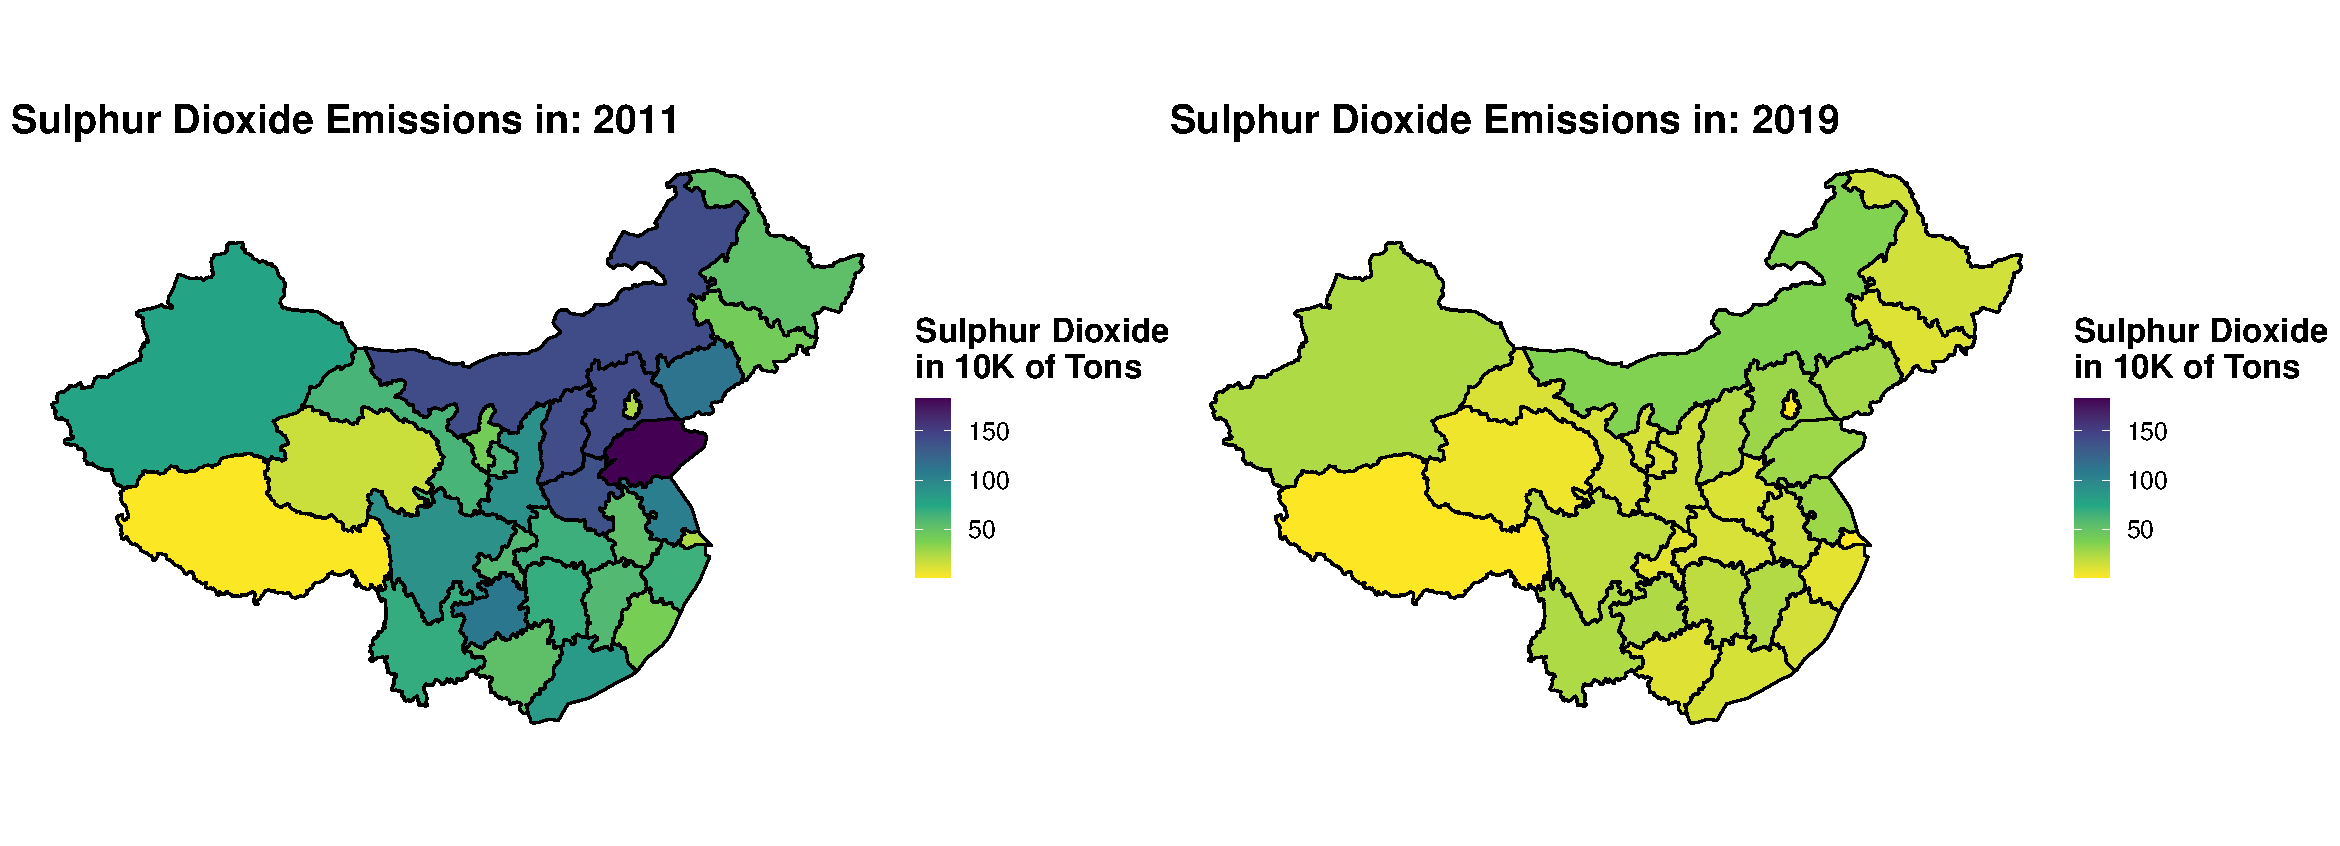
\includegraphics[width = 440pt]{Waste_Gas_Emissions_Sulphur_comp.pdf} 
	\end{center}
	\begin{center}
		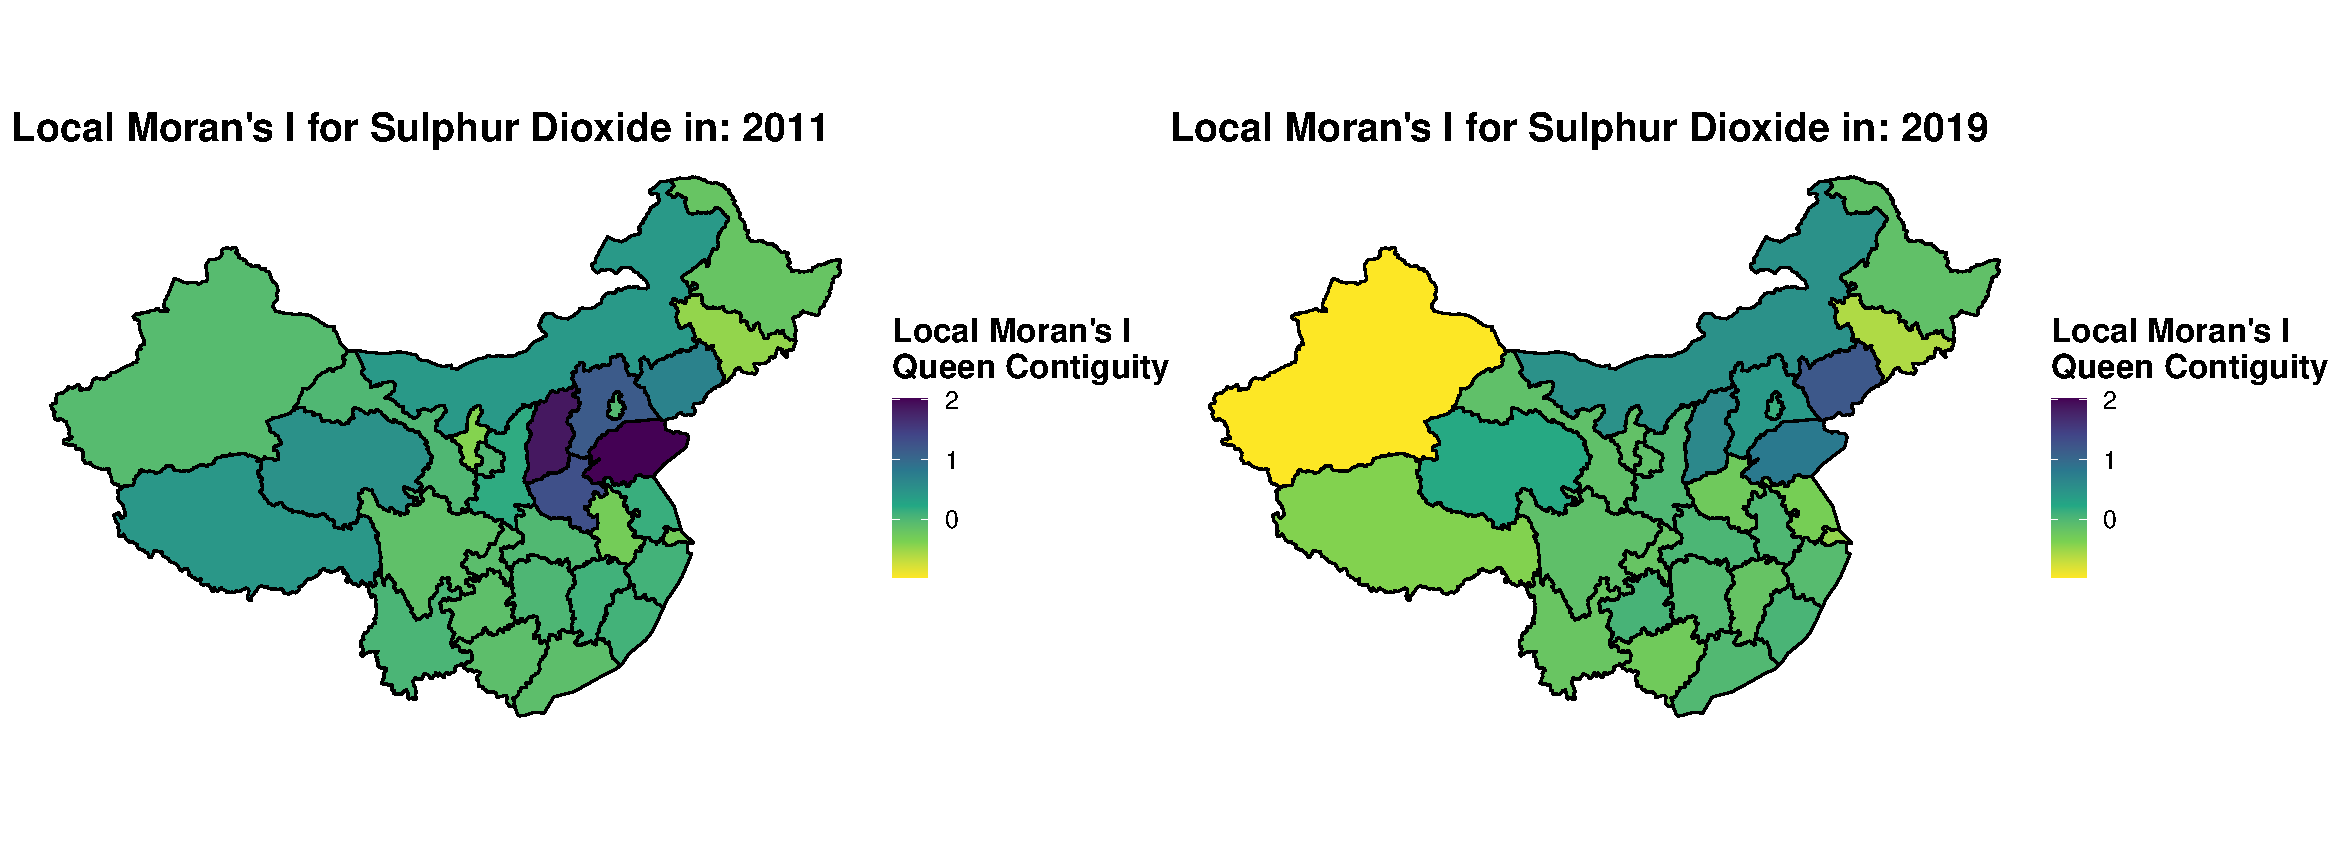
\includegraphics[width = 440pt]{Ii_Waste_Gas_Emissions_Sulphur_comp.pdf} 
	\end{center}
	\subsubsection{Nitrogen Emissions}
		\begin{center}
		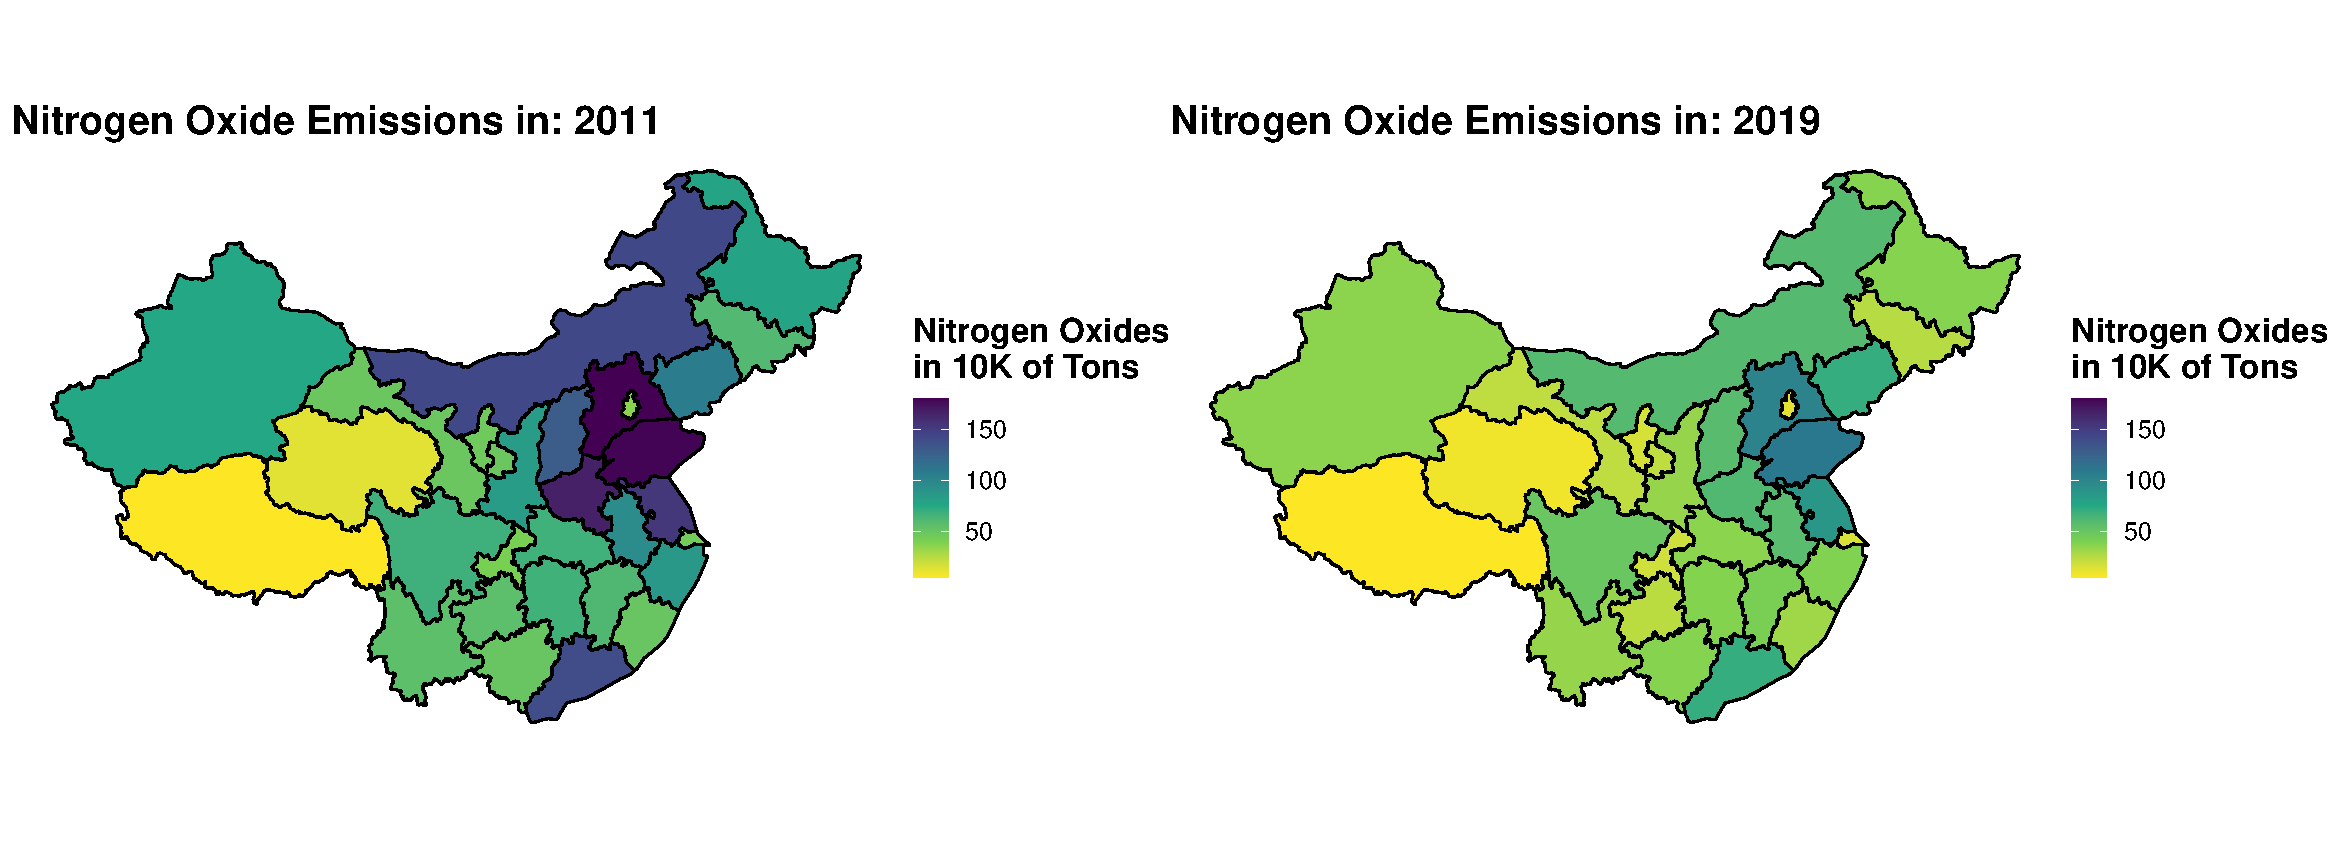
\includegraphics[width = 440pt]{Waste_Gas_Emissions_Nitrogen_comp.pdf} 
	\end{center}
	\begin{center}
		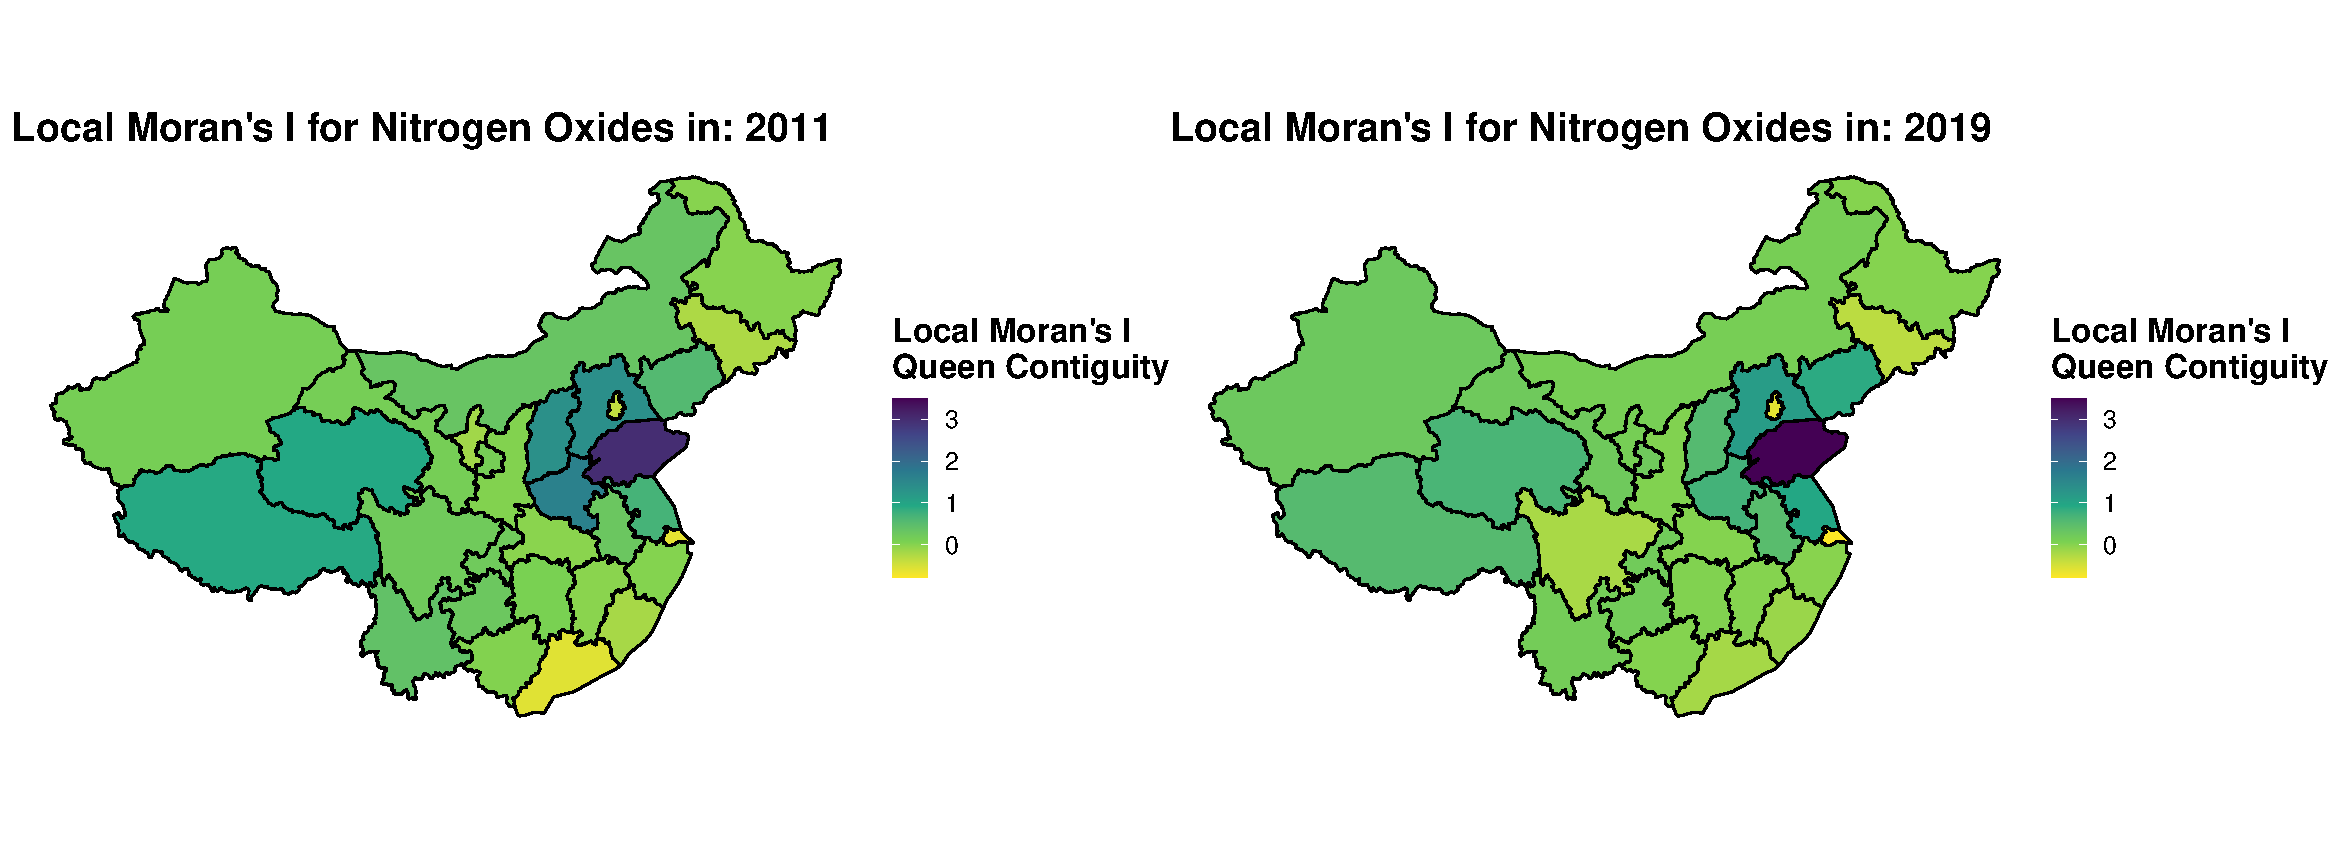
\includegraphics[width = 440pt]{Ii_Waste_Gas_Emissions_Nitrogen_comp.pdf} 
	\end{center}
\end{document}
